\section{Background}
\label{sec:background}
% ============================================================
% This section reviews the background needed for SWEEP-LLM: the two-phase structure of LLM inference, serving-level latency objectives, tensor parallelism, phase disaggregation, GPU frequency scaling, and heterogeneous GPU pools.

% ---------------------------------------------------------------
% \subsubsection*{\normalfont\textbf{LLM Inference Pipeline}}
\subsubsection*{\normalfont\textbf{LLM Inference and Phase Disaggregation}}
\label{sec:bg_pipeline}
% ---------------------------------------------------------------

% The \emph{prefill} phase processes the entire input prompt in a single forward pass through the transformer, producing key-value (KV) cache entries for all input tokens.
% This phase involves large matrix--matrix multiplications and is \emph{compute-bound}: GPU arithmetic units are the bottleneck, and utilization typically exceeds 90\%.
% Prefill latency scales approximately linearly with input length and determines the \emph{time to first token} (TTFT).

% The \emph{decode} phase generates output tokens one at a time.
% Each decode step performs a forward pass that attends to the full KV cache but produces only a single token, resulting in matrix--vector operations that are \emph{memory-bandwidth-bound}: GPU compute units are underutilized (20--40\%), and latency is dominated by the time to read model weights and KV cache from GPU memory.
% The per-token decode latency is measured as \emph{time per output token} (TPOT).
% Modern serving engines such as vLLM~\cite{kwon2023vllm} use \emph{continuous batching} to interleave prefill and decode operations from different requests within the same GPU iteration, improving throughput.
% However, this interleaving means that heavy prefill requests can delay the decode steps of co-located requests, creating interference that must be accounted for in SLO-aware scheduling.

Autoregressive LLM serving has two phases~\cite{agrawal2024taming}. 
In the \emph{prefill} phase, the model processes the input prompt in one forward pass and creates key-value (KV) cache entries for all input tokens. 
Prefill performs large matrix multiplications and is typically compute-bound. 
In the \emph{decode} phase, the model generates output tokens one at a time; each step attends to the existing KV cache while producing a single token, making decode lower-arithmetic-intensity and typically memory-bound. 
This phase asymmetry is the basis for phase-specific placement, parallelism, and frequency choices.

Phase-disaggregated serving exploits this asymmetry by allowing prefill and decode to execute on separate GPU resources, so each phase can use hardware better matched to its bottleneck. 
The benefit is not free: if prefill and decode run on different GPUs, the KV cache produced by prefill must be transferred to the decode GPU. 
This transfer adds latency that grows with prompt length and can offset the benefit of phase specialization. 
A scheduler must therefore balance phase-specific hardware specialization against KV-transfer overhead.

% Autoregressive LLM serving proceeds in two distinct phases~\cite{agrawal2024taming}.
% In the prefill phase, the model processes the entire input prompt in a single forward pass and generates key-value (KV) cache entries for all input tokens.
% Prefill is dominated by large matrix multiplications with high arithmetic intensity and is therefore typically compute-bound.
% In the decode phase, the model generates output tokens one at a time.
% Each decode step attends to the full KV cache while producing only a single token, resulting in lower arithmetic intensity and performance dominated by memory-bandwidth.
% Decode is therefore typically memory-bandwidth-bound, with performance determined more by the memory system than by peak compute throughput.
% Decode is therefore typically memory-bound.
% , with performance determined more by the memory system than by peak arithmetic throughput.
% Modern serving engines such as vLLM~\cite{kwon2023vllm} use continuous batching to interleave work from multiple requests, improving throughput but also creating interference between prefill and decode of co-located requests. Phase disaggregation mitigates this interference by separating the two phases onto different GPU pools.

\begin{figure*}[t]
\vspace{-0.4em}
  \centering
  \begin{minipage}[t]{0.49\textwidth}
    \centering
    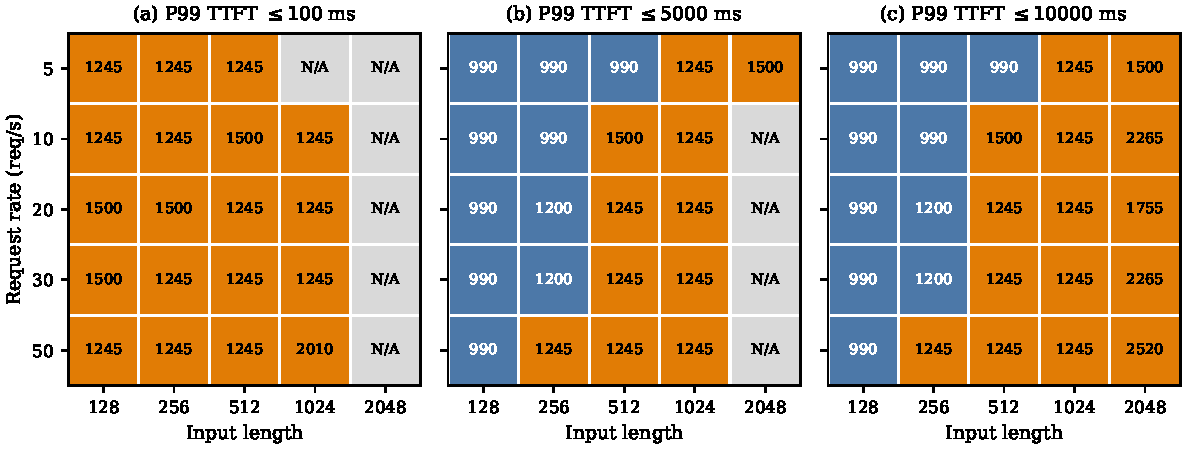
\includegraphics[width=\linewidth]{figures/fig_obs1_prefill_slo_regions_info_to_end_p99.pdf}
  \end{minipage}\hfill
  \begin{minipage}[t]{0.49\textwidth}
    \centering
    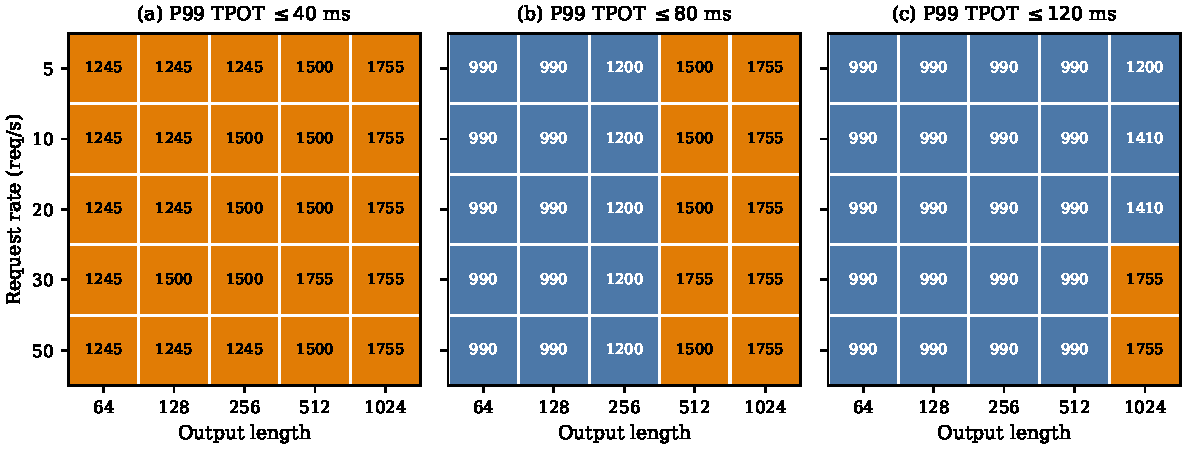
\includegraphics[width=\linewidth]{figures/fig_obs1_decode_slo_regions_info_to_end_p99.pdf}
  \end{minipage}

  {\footnotesize
  \textcolor[rgb]{0.298,0.471,0.659}{\rule{1.2em}{1.2ex}}\ L4 wins\quad
  \textcolor[rgb]{0.882,0.486,0.020}{\rule{1.2em}{1.2ex}}\ L40S wins\quad
  \textcolor[rgb]{0.851,0.851,0.851}{\rule{1.2em}{1.2ex}}\ No feasible config\par}
  \vspace{-0.2em}
  \caption{Phase-specific winner regions on heterogeneous GPUs. Each cell shows the hardware--frequency pair that minimizes energy per request while satisfying the indicated latency bound, with $\mathrm{TP}{=}1$ fixed to isolate hardware--DVFS effects. Cells marked \texttt{N/A} indicate that no measured configuration satisfies the corresponding SLO.}
  \label{fig:obs1-phase-regions}
\end{figure*}

% ---------------------------------------------------------------
\subsubsection*{\normalfont\textbf{Serving-Level Objectives}}
\label{sec:bg_slo}
% ---------------------------------------------------------------

% LLM serving systems are typically governed by latency service-level objectives (SLOs).
% Time to first token (TTFT) measures the delay from request arrival to the first generated token. 
% It is driven mainly by prefill latency and queueing delay, and is critical to interactive responsiveness.
% Time per output token (TPOT) measures the average inter-token latency during decode, which governs the perceived generation speed.
% In this paper, we use both $p_{99}$ TTFT and $p_{99}$ TPOT as SLO constraints, consistent with prior work~\cite{stojkovic2024dynamollm}.
% A configuration is SLO-feasible if its predicted $p_{99}$ TTFT and $p_{99}$ TPOT do not exceed their respective thresholds.

LLM serving systems are commonly constrained by latency service-level objectives (SLOs). 
Time to first token (TTFT) measures the delay from request arrival to the first generated token and is driven mainly by prefill latency and queueing. 
Time per output token (TPOT) measures inter-token decode latency and governs perceived generation speed. 
Following prior work~\cite{stojkovic2024dynamollm}, we use $p_{99}$ TTFT and $p_{99}$ TPOT as the conceptual SLO targets for scheduling decisions.

% DynamoLLM use both P99 TTFT and P99 TBT (TBT = Time Between Tokens, same as TPOT). From their Table IV, they define per-request-type SLOs with separate TTFT and TBT thresholds:
% Short input: TTFT SLO = 250ms, TBT SLO = 100ms
% Medium input: TTFT SLO = 400ms, TBT SLO = 100ms
% Long input: TTFT SLO = 2000ms, TBT SLO = 100ms
% So DynamoLLM is a valid citation for dual-SLO (TTFT + TPOT).
% GreenLLM uses P95

% ---------------------------------------------------------------
\subsubsection*{\normalfont\textbf{Tensor Parallelism}}
\label{sec:bg_tp}
% ---------------------------------------------------------------

Tensor parallelism (TP) partitions a model's weight matrices across multiple GPUs, with each GPU computing a shard of every layer~\cite{kwon2023vllm}.
Increasing TP reduces per-GPU memory demand and can increase aggregate compute and memory bandwidth available to a model instance.
This can reduce per-request latency, particularly when a single GPU's compute or memory capacity is insufficient.
However, higher TP also introduces inter-GPU communication, increases total power draw, and consumes more GPUs per serving instance.
As a result, higher TP can reduce the number of instances that run concurrently, which in turn affects throughput and queueing delay.
% The choice of TP therefore involves a trade-off among latency, throughput, and energy rather than a monotonic performance gain.
The choice of TP therefore involves a trade-off among latency, throughput, and energy rather than providing a monotonic performance gain.
% This trade-off depends on workload conditions and must be coordinated with routing, frequency, and GPU allocation.
This trade-off depends on workload conditions and interacts directly with routing, frequency, and active GPU allocation.

% % ---------------------------------------------------------------
% \subsubsection*{\normalfont\textbf{Disaggregated LLM Serving}}
% \label{sec:bg_disagg}
% % ---------------------------------------------------------------

% Recent LLM serving systems increasingly adopt phase disaggregation, where prefill and decode execute on separate GPUs.
% This design allows each phase to run on hardware that better matches its resource demands.
% When prefill and decode are placed on different GPUs, however, the KV cache generated during prefill must be transferred to the decode GPU.
% % This transfer introduces latency overhead that grows with prompt length and can offset the benefit of phase specialization.
% This transfer introduces latency overhead that grows with prompt length and can offset the benefit of phase specialization.
% % Disaggregation therefore creates a trade-off between hardware specialization and communication overhead, both of which must be considered by the scheduler.
% Disaggregation therefore creates a trade-off between hardware specialization and communication overhead, both of which are relevant when evaluating system-level operating points.

% % ---------------------------------------------------------------
% \subsubsection*{\normalfont\textbf{GPU Frequency Scaling}}
% \label{sec:bg_dvfs}
% % ---------------------------------------------------------------

% Modern GPUs support dynamic voltage and frequency scaling (DVFS), which allows the streaming multiprocessor (SM) clock to be set to different operating points at runtime.
% Lowering the SM frequency reduces power draw, but its performance impact depends on the current bottleneck.
% Compute-bound prefill is generally sensitive to frequency, whereas memory-bound decode is often less affected because its performance is limited primarily by memory bandwidth.
% This phase-dependent sensitivity makes DVFS an important energy-control knob for LLM serving~\cite{ye2025greenllm,patel2025investigating}.
% DVFS on modern GPUs can be applied in milliseconds and can support fine-grained runtime adaptation.

% Modern GPUs support dynamic voltage and frequency scaling (DVFS), allowing the streaming-multiprocessor clock to be adjusted at runtime. 
% Lower frequency reduces power, but its latency impact depends on the bottleneck: compute-bound prefill is generally frequency-sensitive, while memory-bound decode often benefits less from higher SM clocks. 
% This phase-dependent sensitivity makes DVFS a useful energy-control knob for LLM serving~\cite{ye2025greenllm,patel2025investigating}, but also means frequency must be chosen jointly with placement and capacity decisions.

% % ---------------------------------------------------------------
% \subsubsection*{\normalfont\textbf{Heterogeneous GPU Pools}}
% \label{sec:bg_hetero}
% % ---------------------------------------------------------------

% Production serving clusters increasingly combine multiple GPU types to balance cost, performance, and power~\cite{griggs2024melange,jiang2025demystifying}.
% Different GPU types occupy different points in the compute-bandwidth-power design space, so the most energy-efficient choice depends on the phase and workload.
% In general, high-throughput GPUs are better suited to compute-intensive prefill, whereas lower-power GPUs can be attractive for decode when their bandwidth and latency remain sufficient to satisfy the target SLOs.
% This hardware asymmetry means that the energy-optimal GPU type can differ between prefill and decode, and can shift with workload conditions.

% ============================================================
